\documentclass[t, aspectratio=169]{beamer}
\usepackage[utf8]{vietnam}
\usepackage{amsmath,amssymb}
\usepackage{lmodern}
\usepackage{booktabs}
\usepackage{array}
\usepackage{tikz}
\usetikzlibrary{arrows.meta, positioning, calc, fit, shapes.geometric, shapes.symbols}

% --- Cau hinh le cho template HUST ---
\def\slideContentLeftMargin{0.7cm}
\def\slideContentRightMargin{0.9cm}
\def\hustHeaderHeight{1cm}
\def\slideContentBotMargin{3.5cm}

\usepackage[blue, 169]{beamerthemeHUST}

\renewcommand{\titlePageTitleX}{-0.2cm}
\renewcommand{\titlePageTitleY}{-0.45cm}
\renewcommand{\hustTitleAlign}{\alignLeft}
\renewcommand{\hustSubtitleAlign}{\alignLeft}
\renewcommand{\hustAuthorAlign}{\alignLeft}
\renewcommand{\hustInstAlign}{\alignLeft}

\title{CÁC CƠ CHẾ PHÁT HIỆN XÂM NHẬP MẠNG}
\subtitle{Báo cáo bài tập lớn - IT4015 Nhập môn An toàn thông tin}
\author{\texorpdfstring{Nguyễn Đình Tuấn Minh - 20230048\\Vũ Đức Tâm - 20230064\\Nguyễn Gia Khánh - 202416803\\Nguyễn Đăng Cao Tuấn - 202400119}{Nhóm sinh viên}}
\institute{Trường Công nghệ Thông tin và Truyền thông - Đại học Bách khoa Hà Nội\\Giảng viên hướng dẫn: PGS. TS. Nguyễn Linh Giang}
\date{\today}

\definecolor{attackred}{HTML}{CE1628}
\definecolor{detectblue}{HTML}{005A8C}
\definecolor{safegray}{HTML}{F1F3F5}
\definecolor{warnorange}{HTML}{E67700}
\definecolor{goodgreen}{HTML}{2B8A3E}

\setbeamertemplate{itemize item}{\raise0.15ex\hbox{\small$\blacktriangleright$}}
\setbeamertemplate{itemize subitem}{\raise0.1ex\hbox{\scriptsize$\bullet$}}

\tikzset{
    box/.style={rectangle, draw=black!45, fill=white, rounded corners=1.5pt, minimum height=0.8cm, align=center, font=\small},
    bluebox/.style={box, draw=detectblue!70, fill=detectblue!8},
    redbox/.style={box, draw=attackred!70, fill=attackred!8},
    greenbox/.style={box, draw=goodgreen!70, fill=goodgreen!8},
    orangebox/.style={box, draw=warnorange!70, fill=warnorange!10},
    arrow/.style={-{Stealth[length=2mm]}, thick, draw=black!70},
    dashedarrow/.style={-{Stealth[length=2mm]}, thick, dashed, draw=black!65}
}

\newcommand{\metricbox}[3]{
    \begin{tikzpicture}
        \node[draw=#1!70, fill=#1!10, rounded corners=2pt, minimum width=3.1cm, minimum height=1.2cm, align=center] {
            {\Large\bfseries #2}\\[-1pt]{\footnotesize #3}
        };
    \end{tikzpicture}
}

\begin{document}

\hustintropage{IT4015 - Nhập môn An toàn thông tin}
\husttitlepage

\begin{frame}{Nội dung trình bày}
    \tableofcontents[hideallsubsections]
\end{frame}

\resetPageCount
\showPageNumber
\useStyleHustFull
\useThinBar

\section{Bài toán và mục tiêu}

\begin{frame}{Vì sao cần NIDS?}
    \small
    \begin{columns}[T,onlytextwidth]
        \begin{column}{0.43\textwidth}
            \textbf{Bối cảnh}
            \begin{itemize}
                \item Firewall chưa đủ để hiểu toàn bộ traffic behavior.
                \item Attack traffic có thể đi qua HTTP, DNS hoặc internal traffic.
                \item Cần alert sớm để điều tra và phản ứng.
            \end{itemize}

            \vspace{0.25em}
            \textbf{Project objectives}
            \begin{itemize}
                \item Xây dựng NIDS nhỏ gọn bằng Python.
                \item Minh họa hai detection layers: behavior-based và signature-based.
            \end{itemize}
        \end{column}
        \begin{column}{0.56\textwidth}
            \centering
            \resizebox{\linewidth}{!}{%
            \begin{tikzpicture}[node distance=0.6cm and 0.45cm]
                \node[cloud, cloud puffs=10, draw=black!50, fill=safegray, minimum width=1.7cm, minimum height=0.9cm, align=center] (net) {Internet};
                \node[redbox, right=of net, minimum width=2.05cm] (attacker) {Attack\\\footnotesize scan/flood/payload};
                \node[bluebox, right=of attacker, minimum width=2.0cm] (firewall) {Firewall\\\footnotesize lớp lọc ban đầu};
                \node[greenbox, right=of firewall, minimum width=2.05cm] (server) {Dịch vụ\\\footnotesize HTTP/DNS};
                \node[orangebox, below=1.15cm of firewall, minimum width=2.7cm] (nids) {NIDS Sensor\\\footnotesize monitor + alert};
                \node[bluebox, below=1.15cm of server, minimum width=2.7cm] (dashboard) {Dashboard\\\footnotesize alert statistics};

                \draw[arrow] (net) -- (attacker);
                \draw[arrow] (attacker) -- (firewall);
                \draw[arrow] (firewall) -- (server);
                \draw[dashedarrow] (firewall) -- node[left, font=\scriptsize] {mirror/sniff} (nids);
                \draw[arrow] (nids) -- (dashboard);
            \end{tikzpicture}
            }

            \vspace{0.45em}
            \footnotesize NIDS hoạt động thụ động: đọc traffic, phân tích và sinh alert; không chặn trực tiếp như IPS.
        \end{column}
    \end{columns}
\end{frame}

\begin{frame}{Phạm vi triển khai}
    \begin{columns}[T,onlytextwidth]
        \begin{column}{0.33\textwidth}
            \metricbox{detectblue}{PCAP / Live}{data source}
        \end{column}
        \begin{column}{0.33\textwidth}
            \metricbox{attackred}{5 rules}{behavior detection}
        \end{column}
        \begin{column}{0.33\textwidth}
            \metricbox{goodgreen}{3 rules}{HTTP signature demo}
        \end{column}
    \end{columns}

    \vspace{0.7cm}
    \begin{columns}[T,onlytextwidth]
        \begin{column}{0.48\textwidth}
            \textbf{Đã thực hiện}
            \begin{itemize}
                \item Packet capture bằng Scapy.
                \item Chuẩn hóa thành \texttt{PacketEvent}.
                \item Detect port scan, ICMP flood, SYN flood, DNS đáng ngờ, DNS tunneling.
                \item Match Suricata-style rule subset cho HTTP/DNS/payload.
                \item Lưu JSONL và trực quan hóa bằng Flask.
            \end{itemize}
        \end{column}
        \begin{column}{0.48\textwidth}
            \textbf{Giới hạn chủ động đặt ra}
            \begin{itemize}
                \item Không thay thế Suricata, Zeek hoặc IDS production.
                \item Chưa giải mã TLS/HTTPS.
                \item Chưa tái tạo TCP stream đầy đủ.
                \item Detection threshold dùng cấu hình tĩnh để dễ trình diễn.
            \end{itemize}
        \end{column}
    \end{columns}
\end{frame}

\section{Kiến trúc hệ thống}

\begin{frame}{Pipeline xử lý của hệ thống}
    \centering
    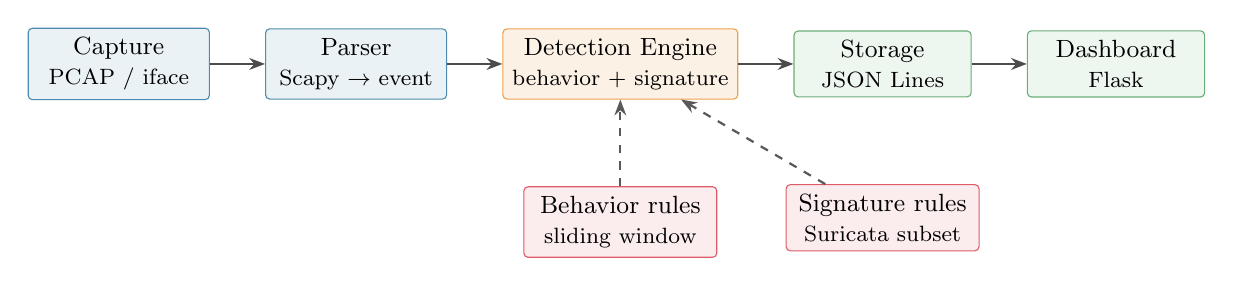
\begin{tikzpicture}[node distance=0.55cm and 0.7cm]
        \node[bluebox, minimum width=2.3cm] (capture) {Capture\\\footnotesize PCAP / iface};
        \node[bluebox, right=of capture, minimum width=2.3cm] (parser) {Parser\\\footnotesize Scapy $\rightarrow$ event};
        \node[orangebox, right=of parser, minimum width=2.7cm] (engine) {Detection Engine\\\footnotesize behavior + signature};
        \node[greenbox, right=of engine, minimum width=2.25cm] (store) {Storage\\\footnotesize JSON Lines};
        \node[greenbox, right=of store, minimum width=2.25cm] (dash) {Dashboard\\\footnotesize Flask};

        \draw[arrow] (capture) -- (parser);
        \draw[arrow] (parser) -- (engine);
        \draw[arrow] (engine) -- (store);
        \draw[arrow] (store) -- (dash);

        \node[redbox, below=1.1cm of engine, minimum width=2.45cm] (rules1) {Behavior rules\\\footnotesize sliding window};
        \node[redbox, below=1.1cm of store, minimum width=2.45cm] (rules2) {Signature rules\\\footnotesize Suricata subset};
        \draw[dashedarrow] (rules1) -- (engine);
        \draw[dashedarrow] (rules2) -- (engine);
    \end{tikzpicture}

    \vspace{0.6cm}
    \begin{block}{Design idea}
        The proposed NIDS follows a CIDF-like IDS pipeline architecture and implements a lightweight Suricata/Snort-style detection model, combining behavior-based detection with signature-based rule matching.
    \end{block}
\end{frame}

\begin{frame}{Proposed Design Simulation}
    \begin{block}{Design statement}
        The proposed NIDS follows a CIDF-like IDS pipeline architecture and implements a lightweight Suricata/Snort-style detection model, combining behavior-based detection with signature-based rule matching.
    \end{block}

    \vspace{0.5cm}
    \begin{columns}[T,onlytextwidth]
        \begin{column}{0.48\textwidth}
            \textbf{CIDF-like pipeline}
            \begin{itemize}
                \item Tách vai trò capture, analysis, storage và visualization.
                \item Mỗi module nhận một data format rõ ràng.
                \item Dễ thay thế PCAP/live traffic source hoặc dashboard.
            \end{itemize}
        \end{column}
        \begin{column}{0.48\textwidth}
            \textbf{Suricata/Snort-style model}
            \begin{itemize}
                \item Rule có header và option.
                \item So khớp payload, HTTP field, DNS query.
                \item Kết hợp với rule behavior dùng time window.
            \end{itemize}
        \end{column}
    \end{columns}
\end{frame}

\begin{frame}{CIDF-like Pipeline Mapping}
    \centering
    \resizebox{0.92\linewidth}{!}{%
    \begin{tikzpicture}[node distance=0.55cm and 0.7cm]
        \node[bluebox, minimum width=2.6cm, minimum height=0.9cm] (eg) {Event Generator\\\footnotesize Scapy capture};
        \node[bluebox, right=of eg, minimum width=2.6cm, minimum height=0.9cm] (norm) {Normalizer\\\footnotesize PacketEvent};
        \node[orangebox, right=of norm, minimum width=2.6cm, minimum height=0.9cm] (ea) {Event Analyzer\\\footnotesize rule engine};
        \node[greenbox, right=of ea, minimum width=2.6cm, minimum height=0.9cm] (edb) {Event DB\\\footnotesize JSONL alerts};
        \node[greenbox, right=of edb, minimum width=2.6cm, minimum height=0.9cm] (ru) {Response Unit\\\footnotesize dashboard};

        \draw[arrow] (eg) -- (norm);
        \draw[arrow] (norm) -- (ea);
        \draw[arrow] (ea) -- (edb);
        \draw[arrow] (edb) -- (ru);

        \node[box, below=0.8cm of norm, text width=3.4cm] (raw) {\footnotesize Raw packet không đưa thẳng vào rule engine};
        \node[box, below=0.8cm of ea, text width=3.4cm] (schema) {\footnotesize Event schema giúp rule dễ test};
        \draw[dashedarrow] (raw) -- (norm);
        \draw[dashedarrow] (schema) -- (ea);
    \end{tikzpicture}
    }
\end{frame}

\begin{frame}{Packet Normalization thành PacketEvent}
    \begin{columns}[T,onlytextwidth]
        \begin{column}{0.48\textwidth}
            \textbf{Vấn đề}
            \begin{itemize}
                \item Raw packet phụ thuộc từng giao thức và thư viện Scapy.
                \item Rule engine cần cùng một schema để đánh giá TCP, ICMP, DNS, HTTP.
                \item Nếu xử lý trực tiếp payload thô, rule sẽ khó viết và khó kiểm thử.
            \end{itemize}

            \vspace{0.5em}
            \textbf{Cách làm}
            \begin{itemize}
                \item Parser rút ra metadata chung: IP, port, protocol, length, TCP flags.
                \item Parser bổ sung trường chuyên biệt: DNS query, HTTP method, URI, Host, User-Agent, payload text.
            \end{itemize}
        \end{column}
        \begin{column}{0.5\textwidth}
            \centering
            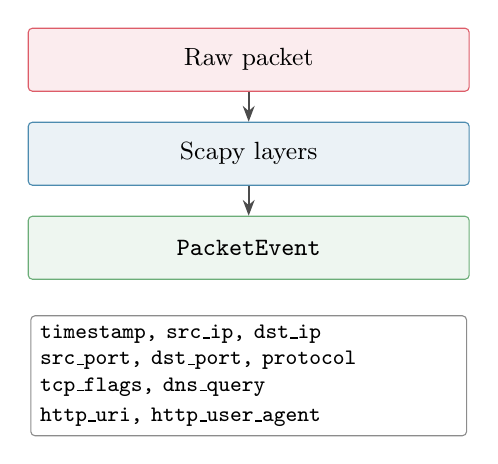
\begin{tikzpicture}[node distance=0.38cm]
                \node[redbox, minimum width=5.6cm] (raw) {Raw packet};
                \node[bluebox, below=of raw, minimum width=5.6cm] (scapy) {Scapy layers};
                \node[greenbox, below=of scapy, minimum width=5.6cm] (event) {\texttt{PacketEvent}};
                \draw[arrow] (raw) -- (scapy);
                \draw[arrow] (scapy) -- (event);
                \node[box, below=0.45cm of event, text width=5.3cm, align=left] {
                    \footnotesize
                    \texttt{timestamp, src\_ip, dst\_ip}\\
                    \texttt{src\_port, dst\_port, protocol}\\
                    \texttt{tcp\_flags, dns\_query}\\
                    \texttt{http\_uri, http\_user\_agent}
                };
            \end{tikzpicture}
        \end{column}
    \end{columns}
\end{frame}

\begin{frame}{Detection Engine: hai lớp detection}
    \begin{columns}[T,onlytextwidth]
        \begin{column}{0.49\textwidth}
            \begin{block}{1. Behavior-based detection}
                \begin{itemize}
                    \item Theo dõi event sequence trong time window.
                    \item Phù hợp với scan, flood, tunneling và frequency anomaly.
                    \item Không cần biết trước payload chính xác.
                \end{itemize}
            \end{block}
        \end{column}
        \begin{column}{0.49\textwidth}
            \begin{alertblock}{2. Signature-based matching}
                \begin{itemize}
                    \item So khớp rule với header, buffer HTTP/DNS/payload.
                    \item Phù hợp với SQL Injection, công cụ tự động, chuỗi độc hại đã biết.
                    \item Alert dễ giải thích bằng evidence.
                \end{itemize}
            \end{alertblock}
        \end{column}
    \end{columns}

    \vspace{0.45cm}
    \centering
    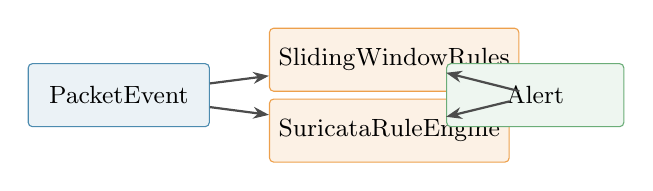
\begin{tikzpicture}[node distance=0.55cm and 0.75cm]
        \node[bluebox, minimum width=2.3cm] (event) {PacketEvent};
        \node[orangebox, right=of event, yshift=0.45cm, minimum width=2.8cm] (behavior) {SlidingWindowRules};
        \node[orangebox, right=of event, yshift=-0.45cm, minimum width=2.8cm] (sig) {SuricataRuleEngine};
        \node[greenbox, right=3.0cm of event, minimum width=2.25cm] (alert) {Alert};
        \draw[arrow] (event) -- (behavior);
        \draw[arrow] (event) -- (sig);
        \draw[arrow] (behavior) -- (alert);
        \draw[arrow] (sig) -- (alert);
    \end{tikzpicture}
\end{frame}

\section{Attack and Detection Mechanisms}

\begin{frame}{Port Scan: principle and detection condition}
    \textbf{Attack mechanism}
    \begin{itemize}
        \item Attacker gửi probe TCP tới nhiều cổng của cùng mục tiêu.
        \item Mục tiêu là identify open services: SSH, HTTP, SMB, database.
        \item Đây thường là bước tiền khai thác trước khi chọn lỗ hổng cụ thể.
    \end{itemize}

    \vspace{0.55em}
    \textbf{Detection condition trong đồ án}
    \begin{itemize}
        \item Một source chạm \textbf{20 unique TCP destination ports trong 10 giây}.
        \item Chỉ đếm các flag probe: SYN, FIN, NULL, XMAS, ACK.
        \item Không đếm response packets như RST hoặc SYN-ACK để giảm false positive.
    \end{itemize}
\end{frame}

\begin{frame}{Port Scan: probe flow}
    \centering
    \resizebox{0.88\linewidth}{!}{%
    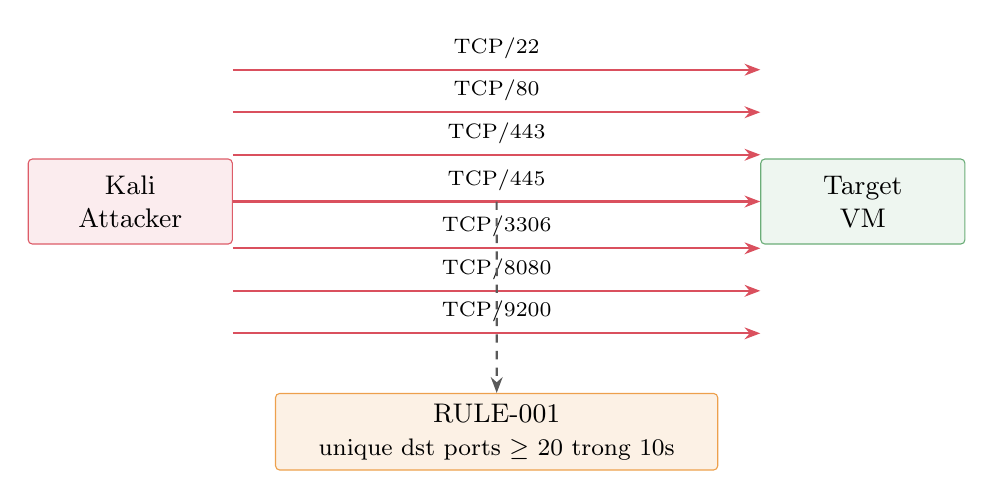
\begin{tikzpicture}[scale=1.08, transform shape]
        \node[redbox, minimum width=2.4cm, minimum height=1.0cm] (atk) {Kali\\Attacker};
        \node[greenbox, right=6.2cm of atk, minimum width=2.4cm, minimum height=1.0cm] (victim) {Target\\VM};
        \foreach \y/\p in {1.55/22,1.05/80,0.55/443,0/445,-0.55/3306,-1.05/8080,-1.55/9200} {
            \draw[arrow, draw=attackred!75] ([yshift=\y cm]atk.east) -- node[above, sloped, font=\scriptsize] {TCP/\p} ([yshift=\y cm]victim.west);
        }
        \node[orangebox, below=2.25cm of $(atk)!0.5!(victim)$, minimum width=5.2cm, minimum height=0.9cm] (rule) {RULE-001\\\footnotesize unique dst ports $\geq$ 20 trong 10s};
        \draw[dashedarrow] ($(atk)!0.5!(victim)$) -- (rule);
    \end{tikzpicture}
    }
\end{frame}

\begin{frame}{Flood: principle and detection threshold}
    \begin{columns}[T,onlytextwidth]
        \begin{column}{0.48\textwidth}
            \begin{block}{ICMP Ping Flood}
                \begin{itemize}
                    \item Gửi nhiều Echo Request để tiêu tốn băng thông hoặc CPU xử lý.
                    \item Rule chỉ đếm request-side: type 8, 13, 17.
                    \item Demo threshold: \textbf{100 packets / 10 seconds}.
                \end{itemize}
            \end{block}
        \end{column}
        \begin{column}{0.48\textwidth}
            \begin{alertblock}{TCP SYN Flood}
                \begin{itemize}
                    \item Gửi nhiều SYN để tạo trạng thái kết nối chưa hoàn tất.
                    \item Rule đếm packet có TCP flag đúng bằng \texttt{S}.
                    \item Demo threshold: \textbf{100 SYN / 10 seconds}.
                \end{itemize}
            \end{alertblock}
        \end{column}
    \end{columns}
\end{frame}

\begin{frame}{Flood: threshold crossing over time}
    \centering
    \resizebox{0.86\linewidth}{!}{%
    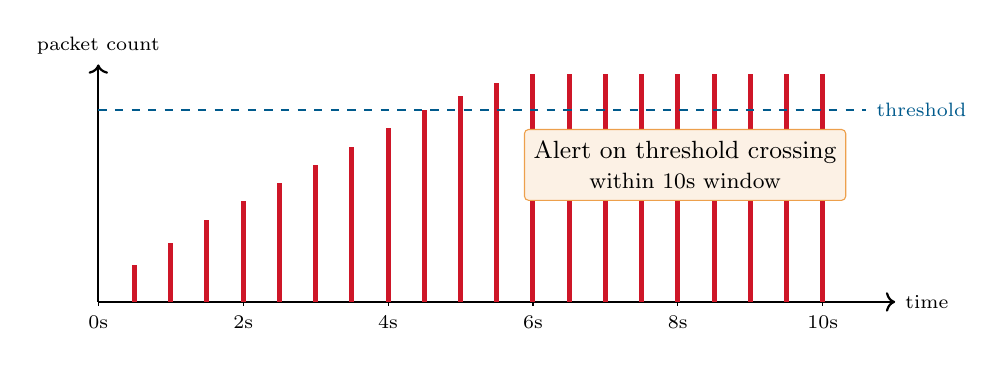
\begin{tikzpicture}[x=0.92cm, y=0.58cm]
        \draw[->, thick] (0,0) -- (11,0) node[right, font=\scriptsize] {time};
        \draw[->, thick] (0,0) -- (0,5.2) node[above, font=\scriptsize] {packet count};
        \foreach \x/\lab in {0/0s,2/2s,4/4s,6/6s,8/8s,10/10s}
            \draw (\x,0.1) -- (\x,-0.1) node[below, font=\scriptsize] {\lab};
        \foreach \x/\h in {0.5/0.8,1/1.3,1.5/1.8,2/2.2,2.5/2.6,3/3.0,3.5/3.4,4/3.8,4.5/4.2,5/4.5,5.5/4.8,6/5.0,6.5/5.0,7/5.0,7.5/5.0,8/5.0,8.5/5.0,9/5.0,9.5/5.0,10/5.0}
            \draw[attackred, line width=1.8pt] (\x,0) -- (\x,\h);
        \draw[dashed, detectblue, thick] (0,4.2) -- (10.6,4.2) node[right, font=\scriptsize] {threshold};
        \node[orangebox, minimum width=3.2cm, minimum height=0.9cm] at (8.1,3.0) {Alert on threshold crossing\\\footnotesize within 10s window};
    \end{tikzpicture}
    }
\end{frame}

\begin{frame}{DNS Anomaly: principle and formula}
    \textbf{Attack mechanism}
    \begin{itemize}
        \item DNS thường được phép đi qua firewall nên có thể bị lợi dụng làm kênh phụ.
        \item Attacker có thể query malicious domain hoặc nhúng data vào DNS label.
        \item Encoded/base64 data thường tạo long label, khó đọc và entropy cao.
    \end{itemize}

    \vspace{0.6em}
    \textbf{Shannon entropy dùng để đánh giá label}
    \[
        H(X) = -\sum_i p(x_i)\log_2 p(x_i)
    \]
    \begin{itemize}
        \item Label đủ dài và có entropy $\geq 3.8$ được xem là chỉ báo tunneling.
        \item RULE-005 tạo alert khi có ít nhất 5 anomalous queries trong 30 giây.
    \end{itemize}
\end{frame}

\begin{frame}{DNS Anomaly: rule diagram}
    \centering
    \resizebox{0.58\linewidth}{!}{%
    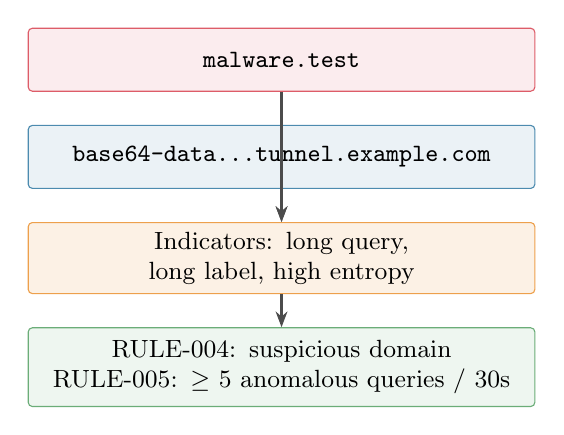
\begin{tikzpicture}[node distance=0.42cm]
        \node[redbox, text width=6.2cm, minimum height=0.8cm] (q1) {\texttt{malware.test}};
        \node[bluebox, below=of q1, text width=6.2cm, minimum height=0.8cm] (q2) {\texttt{base64-data...tunnel.example.com}};
        \node[orangebox, below=of q2, text width=6.2cm, minimum height=0.8cm] (features) {
            Indicators: long query, long label, high entropy
        };
        \node[greenbox, below=of features, text width=6.2cm, minimum height=1.0cm] (alert) {
            RULE-004: suspicious domain\\
            RULE-005: $\geq$ 5 anomalous queries / 30s
        };
        \draw[arrow] (q1) -- (features);
        \draw[arrow] (q2) -- (features);
        \draw[arrow] (features) -- (alert);
    \end{tikzpicture}
    }
\end{frame}

\begin{frame}{HTTP Signature: rule and example}
    \textbf{Demo rules}
    \begin{itemize}
        \item SQL Injection trong HTTP URI.
        \item User-Agent chứa \texttt{sqlmap}.
        \item SQL Injection trong body POST hoặc payload thô.
    \end{itemize}

    \vspace{0.6em}
    \textbf{Rule example}
    \begin{block}{Suricata-style}
        \footnotesize
        \texttt{alert http any any -> any 80}\\
        \texttt{(msg:"sqlmap Scanner User-Agent Detected";}\\
        \texttt{http.user\_agent; content:"sqlmap"; nocase;}\\
        \texttt{classtype:attempted-recon; priority:2; sid:1000002; rev:1;)}
    \end{block}
\end{frame}

\begin{frame}{HTTP Signature: sticky buffer diagram}
    \centering
    \resizebox{0.76\linewidth}{!}{%
    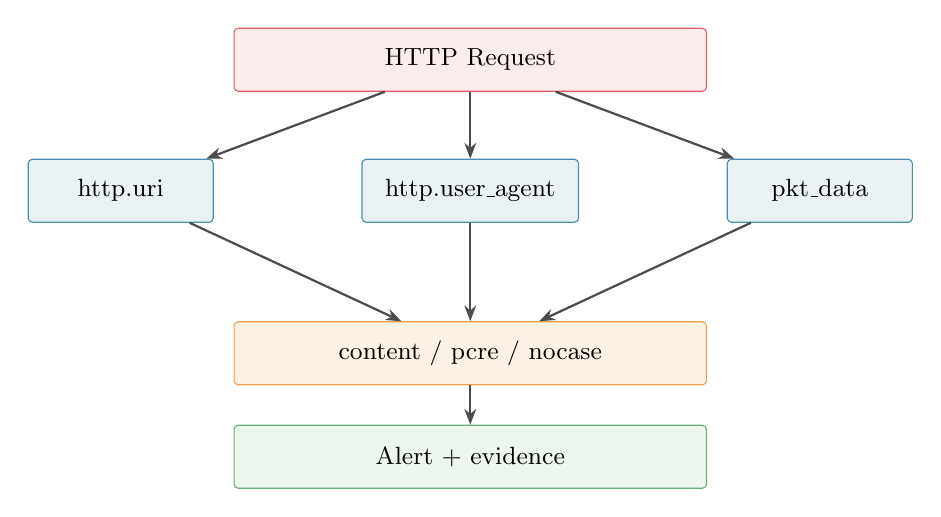
\begin{tikzpicture}[node distance=0.5cm]
        \node[redbox, minimum width=6.0cm, minimum height=0.8cm] (req) {HTTP Request};
        \node[bluebox, below left=0.85cm and 0.25cm of req, minimum width=2.35cm] (uri) {http.uri};
        \node[bluebox, below=0.85cm of req, minimum width=2.75cm] (ua) {http.user\_agent};
        \node[bluebox, below right=0.85cm and 0.25cm of req, minimum width=2.35cm] (body) {pkt\_data};
        \node[orangebox, below=1.25cm of ua, minimum width=6.0cm, minimum height=0.8cm] (match) {content / pcre / nocase};
        \node[greenbox, below=of match, minimum width=6.0cm, minimum height=0.8cm] (alert) {Alert + evidence};
        \draw[arrow] (req) -- (uri);
        \draw[arrow] (req) -- (ua);
        \draw[arrow] (req) -- (body);
        \draw[arrow] (uri) -- (match);
        \draw[arrow] (ua) -- (match);
        \draw[arrow] (body) -- (match);
        \draw[arrow] (match) -- (alert);
    \end{tikzpicture}
    }
\end{frame}

\section{IDS Design Simulation}

\begin{frame}{Simulation Scope trong đồ án}
    \textbf{Không xây dựng IDS production}
    \begin{itemize}
        \item Mục tiêu là simulate các core functional blocks của một NIDS.
        \item Ưu tiên readability, demoability và testability hơn high performance.
        \item Mỗi alert cần có rule ID, description và evidence để giải thích được.
    \end{itemize}

    \vspace{0.55em}
    \textbf{Hai detection layers được simulate}
    \begin{itemize}
        \item Behavior-based detection: detect anomaly theo frequency, time window và entropy.
        \item Signature-based matching: simulate cách Snort/Suricata dùng rule để match header, buffer và content.
    \end{itemize}
\end{frame}

\begin{frame}{Snort/Suricata-style Rule Model}
    \centering
    \resizebox{0.88\linewidth}{!}{%
    \begin{tikzpicture}[node distance=0.55cm]
        \node[redbox, text width=8.2cm, minimum height=0.85cm] (rule) {
            \texttt{alert http any any -> any 80 (msg; http.user\_agent; content; sid;)}
        };
        \node[bluebox, below left=0.85cm and 0.15cm of rule, text width=3.5cm] (header) {
            Header\\\footnotesize action, protocol, IP, port, direction
        };
        \node[orangebox, below right=0.85cm and 0.15cm of rule, text width=3.5cm] (opts) {
            Options\\\footnotesize msg, sid, priority, buffer, content
        };
        \node[greenbox, below=1.85cm of rule, text width=7.2cm] (match) {
            Match khi header đúng và tất cả option conditions thỏa mãn
        };
        \draw[arrow] (rule) -- (header);
        \draw[arrow] (rule) -- (opts);
        \draw[arrow] (header) -- (match);
        \draw[arrow] (opts) -- (match);
    \end{tikzpicture}
    }
\end{frame}

\begin{frame}{Behavior + Signature Fusion Flow}
    \centering
    \resizebox{0.9\linewidth}{!}{%
    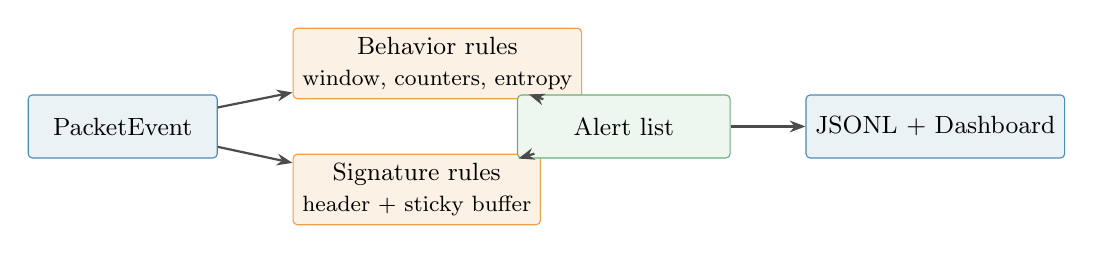
\begin{tikzpicture}[node distance=0.62cm and 0.95cm]
        \node[bluebox, minimum width=2.4cm] (event) {PacketEvent};
        \node[orangebox, right=of event, yshift=0.8cm, minimum width=3.1cm] (behavior) {Behavior rules\\\footnotesize window, counters, entropy};
        \node[orangebox, right=of event, yshift=-0.8cm, minimum width=3.1cm] (signature) {Signature rules\\\footnotesize header + sticky buffer};
        \node[greenbox, right=3.8cm of event, minimum width=2.7cm] (alerts) {Alert list};
        \node[bluebox, right=of alerts, minimum width=2.7cm] (store) {JSONL + Dashboard};

        \draw[arrow] (event) -- (behavior);
        \draw[arrow] (event) -- (signature);
        \draw[arrow] (behavior) -- (alerts);
        \draw[arrow] (signature) -- (alerts);
        \draw[arrow] (alerts) -- (store);
    \end{tikzpicture}
    }

    \vspace{0.45cm}
    \begin{block}{Ý nghĩa}
        Behavior rules bắt anomaly patterns theo time series; signature rules bắt known payload hoặc application fields. Hai nhánh cùng sinh ra một \texttt{Alert} format.
    \end{block}
\end{frame}

\begin{frame}{Alert Format và Evidence}
    \begin{columns}[T,onlytextwidth]
        \begin{column}{0.48\textwidth}
            \textbf{Main alert fields}
            \begin{itemize}
                \item \texttt{rule\_id}: rule identifier.
                \item \texttt{attack\_type}: attack type.
                \item \texttt{severity}: mức độ nghiêm trọng.
                \item \texttt{source\_ip}, \texttt{destination\_ip}.
                \item \texttt{description}: short description.
                \item \texttt{evidence}: explanatory data.
            \end{itemize}
        \end{column}
        \begin{column}{0.49\textwidth}
            \begin{block}{Evidence example}
                \footnotesize
                \texttt{\{}\\
                \texttt{\ \ "unique\_ports": [22, 80, 443],}\\
                \texttt{\ \ "count": 20}\\
                \texttt{\}}
            \end{block}

            \vspace{0.35em}
            \begin{block}{Vai trò}
                Evidence giúp người xem dashboard hiểu vì sao rule được kích hoạt, thay vì chỉ thấy một alert label.
            \end{block}
        \end{column}
    \end{columns}
\end{frame}

\begin{frame}{Sliding Window: nguyên lý}
    \textbf{Idea}
    \begin{itemize}
        \item Mỗi source có một queue chứa recent events.
        \item Khi event mới đến, hệ thống drop expired data.
        \item Nếu count hoặc feature vượt threshold thì tạo alert.
    \end{itemize}

    \vspace{0.65em}
    \textbf{Benefits}
    \begin{itemize}
        \item Dễ giải thích bằng evidence trong alert.
        \item Memory cost giới hạn theo số source và time-window length.
        \item Phù hợp để illustrate scan, flood và DNS tunneling.
    \end{itemize}
\end{frame}

\begin{frame}{Sliding Window: timeline}
    \centering
    \resizebox{0.88\linewidth}{!}{%
    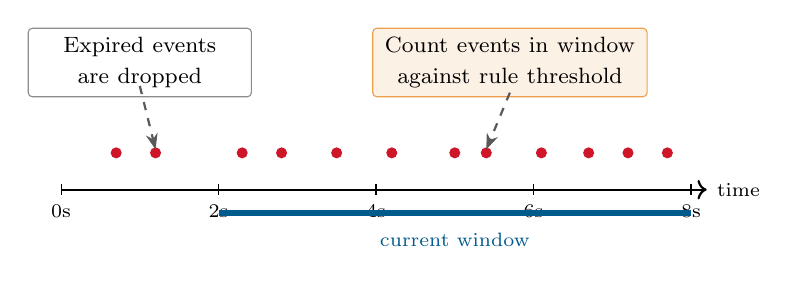
\begin{tikzpicture}[x=1.0cm, y=0.85cm]
        \draw[->, thick] (0,0) -- (8.2,0) node[right, font=\scriptsize] {time};
        \foreach \x/\lab in {0/0,2/2,4/4,6/6,8/8}
            \draw (\x,0.08) -- (\x,-0.08) node[below, font=\scriptsize] {\lab s};
        \draw[detectblue, line width=2pt] (2,-0.35) -- (8,-0.35);
        \node[font=\scriptsize, detectblue] at (5,-0.75) {current window};
        \foreach \x in {0.7,1.2,2.3,2.8,3.5,4.2,5.0,5.4,6.1,6.7,7.2,7.7}
            \fill[attackred] (\x,0.55) circle (2pt);
        \node[box, text width=2.6cm] at (1.0,1.9) {\footnotesize Expired events are dropped};
        \draw[dashedarrow] (1.0,1.55) -- (1.2,0.6);
        \node[orangebox, text width=3.25cm] at (5.7,1.9) {\footnotesize Count events in window\\against rule threshold};
        \draw[dashedarrow] (5.7,1.45) -- (5.4,0.6);
    \end{tikzpicture}
    }
\end{frame}

\begin{frame}{False Positive Reduction bằng Context Filtering}
    \small
    \begin{columns}[T,onlytextwidth]
        \begin{column}{0.5\textwidth}
            \textbf{Port scan}
            \begin{itemize}
                \item Chỉ đếm flag probe: \texttt{S}, \texttt{F}, NULL, \texttt{FPU}, \texttt{A}.
                \item Không đếm RST, SYN-ACK, FIN-ACK vì thường là response packets.
            \end{itemize}
        \end{column}
        \begin{column}{0.48\textwidth}
            \textbf{ICMP flood}
            \begin{itemize}
                \item Chỉ đếm request-side: Echo, Timestamp, Address Mask Request.
                \item Không đếm Echo Reply để tránh gắn nhầm flood source cho target.
            \end{itemize}

            \vspace{0.4em}
            \textbf{Alert cooldown}
            \begin{itemize}
                \item Cùng một rule và cùng một key chỉ re-alert sau 5 giây.
                \item Dashboard không bị ngập bởi duplicate alerts.
            \end{itemize}
        \end{column}
    \end{columns}

    \vspace{0.25cm}
    \centering
    \resizebox{0.82\linewidth}{!}{%
    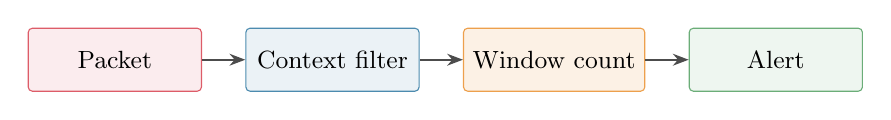
\begin{tikzpicture}[node distance=0.42cm and 0.55cm]
        \node[redbox, minimum width=2.2cm] (packet) {Packet};
        \node[bluebox, right=of packet, minimum width=2.2cm] (context) {Context filter};
        \node[orangebox, right=of context, minimum width=2.2cm] (window) {Window count};
        \node[greenbox, right=of window, minimum width=2.2cm] (alert) {Alert};
        \draw[arrow] (packet) -- (context);
        \draw[arrow] (context) -- (window);
        \draw[arrow] (window) -- (alert);
    \end{tikzpicture}
    }
\end{frame}

\begin{frame}{Suricata-style Signature Engine Subset}
    \begin{columns}[T,onlytextwidth]
        \begin{column}{0.44\textwidth}
            \textbf{Rule components}
            \begin{itemize}
                \item Header: action, protocol, IP, port, direction.
                \item Options: \texttt{msg}, \texttt{sid}, \texttt{priority}, \texttt{content}, \texttt{pcre}.
                \item Sticky buffers: \texttt{pkt\_data}, \texttt{raw\_data}, \texttt{dns.query}, HTTP fields.
            \end{itemize}
        \end{column}
        \begin{column}{0.54\textwidth}
            \centering
            \resizebox{\linewidth}{!}{%
            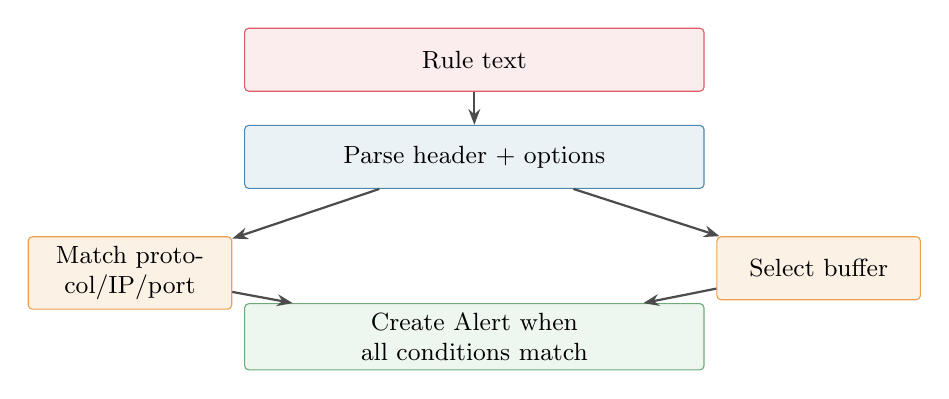
\begin{tikzpicture}[node distance=0.42cm]
                \node[redbox, text width=5.6cm] (text) {Rule text};
                \node[bluebox, below=of text, text width=5.6cm] (parse) {Parse header + options};
                \node[orangebox, below left=0.6cm and 0.15cm of parse, text width=2.35cm] (hdr) {Match protocol/IP/port};
                \node[orangebox, below right=0.6cm and 0.15cm of parse, text width=2.35cm] (buf) {Select buffer};
                \node[greenbox, below=1.45cm of parse, text width=5.6cm] (out) {Create Alert when all conditions match};
                \draw[arrow] (text) -- (parse);
                \draw[arrow] (parse) -- (hdr);
                \draw[arrow] (parse) -- (buf);
                \draw[arrow] (hdr) -- (out);
                \draw[arrow] (buf) -- (out);
            \end{tikzpicture}
            }
        \end{column}
    \end{columns}
\end{frame}

\section{Demo và đánh giá}

\begin{frame}{Mô hình lab kiểm thử}
    \centering
    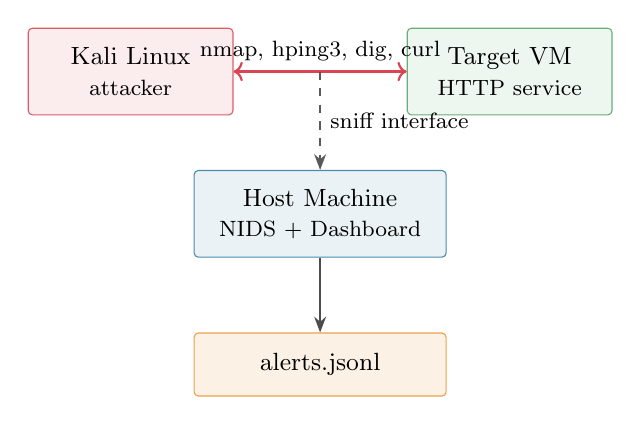
\begin{tikzpicture}[node distance=1.0cm and 2.2cm]
        \node[redbox, minimum width=2.6cm, minimum height=1.1cm] (kali) {Kali Linux\\\footnotesize attacker};
        \node[greenbox, right=of kali, minimum width=2.6cm, minimum height=1.1cm] (target) {Target VM\\\footnotesize HTTP service};
        \node[bluebox, below=1.25cm of $(kali)!0.5!(target)$, minimum width=3.2cm, minimum height=1.1cm] (host) {Host Machine\\\footnotesize NIDS + Dashboard};
        \node[orangebox, below=0.95cm of host, minimum width=3.2cm] (json) {alerts.jsonl};

        \draw[<->, thick, draw=attackred!80] (kali) -- node[above, font=\footnotesize] {nmap, hping3, dig, curl} (target);
        \draw[dashedarrow] ($(kali)!0.5!(target)$) -- node[right, font=\footnotesize] {sniff interface} (host);
        \draw[arrow] (host) -- (json);
    \end{tikzpicture}

    \vspace{0.6cm}
    \begin{block}{Demo objective}
        Chứng minh cùng một pipeline có thể detection cả anomaly theo tần suất và payload khớp signature, sau đó hiển thị thống kê alert trên dashboard.
    \end{block}
\end{frame}

\begin{frame}{Demo scenarios and corresponding rules}
    \centering
    \renewcommand{\arraystretch}{1.25}
    \begin{tabular}{p{3.0cm}p{4.6cm}p{3.5cm}p{2.1cm}}
        \toprule
        \textbf{Scenario} & \textbf{Attack mechanism} & \textbf{Detection signal} & \textbf{Rule} \\
        \midrule
        Port scan & Nmap probes multiple TCP ports & $\geq$ 20 ports / 10s & RULE-001 \\
        ICMP flood & Many Echo Requests & $\geq$ 100 packets / 10s & RULE-002 \\
        SYN flood & Many TCP SYN packets to port 80 & $\geq$ 100 SYN / 10s & RULE-003 \\
        Suspicious DNS & Domain query in blacklist & exact/subdomain match & RULE-004 \\
        DNS tunneling & Long label, high entropy & $\geq$ 5 queries / 30s & RULE-005 \\
        HTTP attack & URI/User-Agent/body contains malicious pattern & content match & custom.rules \\
        \bottomrule
    \end{tabular}
\end{frame}

\begin{frame}{Alert result visualization}
    \begin{columns}[T,onlytextwidth]
        \begin{column}{0.53\textwidth}
            \centering
            \begin{tikzpicture}[x=0.78cm, y=0.45cm]
                \draw[->, thick] (0,0) -- (0,6.2) node[above, font=\scriptsize] {alert categories};
                \draw[->, thick] (0,0) -- (8.5,0);
                \foreach \name/\x/\h/\col in {Scan/0.8/4.0/detectblue,ICMP/2.0/3.5/attackred,SYN/3.2/3.5/attackred,DNS/4.4/2.8/warnorange,Tunnel/5.6/2.4/warnorange,HTTP/6.8/3.2/goodgreen} {
                    \fill[\col!70] (\x,0) rectangle +(0.75,\h);
                    \node[rotate=35, anchor=east, font=\scriptsize] at (\x+0.55,-0.15) {\name};
                }
                \node[box, text width=3.4cm] at (4.8,5.35) {\footnotesize Dashboard tổng hợp theo severity, source IP và danh sách alert gần nhất.};
            \end{tikzpicture}
        \end{column}
        \begin{column}{0.45\textwidth}
            \textbf{Kết quả mong đợi trong lab}
            \begin{itemize}
                \item Terminal NIDS prints alerts in real time.
                \item File JSONL append từng alert độc lập.
                \item Dashboard hiển thị tổng alert, severity, top source IP và alert gần nhất.
            \end{itemize}

            \vspace{0.5em}
            \textbf{Ý nghĩa đánh giá}
            \begin{itemize}
                \item Kiểm chứng đủ hai lớp detection.
                \item Chứng minh data đi hết pipeline từ capture tới dashboard.
            \end{itemize}
        \end{column}
    \end{columns}
\end{frame}

\begin{frame}{Technical evaluation}
    \begin{columns}[T,onlytextwidth]
        \begin{column}{0.49\textwidth}
            \begin{block}{Điểm đạt được}
                \begin{itemize}
                    \item Kiến trúc module rõ: capture, parser, engine, storage, dashboard.
                    \item Rule behavior giải thích được bằng threshold và evidence.
                    \item Rule signature bám theo cú pháp Suricata quen thuộc.
                    \item Có unit test cho parser/rule engine và script demo.
                \end{itemize}
            \end{block}
        \end{column}
        \begin{column}{0.49\textwidth}
            \begin{alertblock}{Hạn chế}
                \begin{itemize}
                    \item Không phân tích payload trong TLS/HTTPS.
                    \item Payload chia nhỏ qua nhiều TCP segment có thể bị bỏ sót.
                    \item Chưa đo false positive/false negative trên dataset lớn.
                    \item Python + Scapy phù hợp demo hơn môi trường tốc độ cao.
                \end{itemize}
            \end{alertblock}
        \end{column}
    \end{columns}
\end{frame}

\section{Kết luận}

\begin{frame}{Kết luận và hướng phát triển}
    \begin{columns}[T,onlytextwidth]
        \begin{column}{0.48\textwidth}
            \textbf{Kết luận}
            \begin{itemize}
                \item Đồ án illustrates một NIDS hoàn chỉnh ở mức học tập.
                \item Hai cơ chế detection bổ sung cho nhau: behavior detection anomaly, signature detection mẫu đã biết.
                \item Dashboard giúp biến alert thô thành thông tin quan sát được.
            \end{itemize}
        \end{column}
        \begin{column}{0.5\textwidth}
            \textbf{Hướng phát triển}
            \begin{itemize}
                \item TCP stream reassembly để so khớp payload theo phiên.
                \item Mở rộng tương thích Suricata rule.
                \item Cấu hình threshold/rule qua YAML hoặc dashboard.
                \item Đo hiệu năng trên PCAP lớn và đánh giá false positive.
                \item Tích hợp webhook hoặc danh sách chặn trong lab.
            \end{itemize}
        \end{column}
    \end{columns}
\end{frame}

\hustcontactpage{\hfill THÔNG TIN ĐỒ ÁN \hfill}{
    \textbf{Đề tài:} Các cơ chế detection xâm nhập mạng\\
    \textbf{Học phần:} IT4015 - Nhập môn An toàn thông tin\\
    \textbf{Giảng viên hướng dẫn:} PGS. TS. Nguyễn Linh Giang\\[0.35cm]
    \textbf{Nhóm sinh viên:}\\
    Nguyễn Đình Tuấn Minh - 20230048\\
    Vũ Đức Tâm - 20230064\\
    Nguyễn Gia Khánh - 202416803\\
    Nguyễn Đăng Cao Tuấn - 202400119\\[0.35cm]
    \textit{Xin chân thành cảm ơn thầy và các bạn đã lắng nghe!}
}

\useStyleLogoOnly
\setbeamertemplate{bibliography item}[text]
\begin{frame}{Tài liệu tham khảo}
    \begin{thebibliography}{9}
        \bibitem{suricata}
        Open Information Security Foundation, \emph{Suricata User Guide}.

        \bibitem{scapy}
        Scapy Project, \emph{Scapy Documentation}.

        \bibitem{nmap}
        Gordon Lyon, \emph{Nmap Network Scanning}.

        \bibitem{project}
        Nhóm sinh viên, \emph{Báo cáo đồ án: Các cơ chế detection xâm nhập mạng}, 2026.
    \end{thebibliography}
\end{frame}

\hustthankyou

\end{document}
